\documentclass[12pt,aspectratio=169]{beamer}
\usetheme{metropolis}
\setbeamersize{text margin left=.5cm,text margin right=.5cm}
\usepackage[lf]{carlito}
\usepackage{tikz}
\usepackage{mathpazo}
\usepackage{xcolor,colortbl}
\usepackage{siunitx}
\usepackage{circuitikz}
\usepackage{mathtools}
\usepackage{bm}
\usepackage[ISO]{diffcoeff}
\diffdef{}{ op-symbol=\mathsf{d} }

\setlength{\parskip}{0pt}
\renewcommand{\baselinestretch}{1}

\usetikzlibrary{patterns}

\sisetup{
  inter-unit-product=\cdot,
  per-mode=symbol
}
\tikzset{
  voltage dir=RP,
  >=latex
}

\title{Topic 14: Magnetism}
\subtitle{AP Physics 2}
\author[TML]{Dr.\ Timothy Leung}
\institute{Olympiads School}
\date{\today}


\newcommand{\pic}[2]{\includegraphics[width=#1\textwidth]{#2}}
\newcommand{\eq}[2]{\vspace{#1}{\Large\begin{displaymath}#2\end{displaymath}}}

\begin{document}

\begin{frame}
  \maketitle
\end{frame}


\begin{frame}{An Electromagnet}
  A popular experiment in magnetism in elementary schools:
  \begin{itemize}
  \item Wrap a copper wire around an iron nail/screw
  \item Connect the ends of the wire to a battery
  \item When the circuit is closed, the nail becomes magnetized, picks up
    small paper clips
  \item As soon as the current stops, the nail stops being magnetic
  \end{itemize}
  \begin{center}
    \pic{.4}{nail}
  \end{center}
\end{frame}


\section{Magnetism}

\begin{frame}{Review of Magnetic Field}
  \begin{itemize}
  \item Magnetism is generated by moving charged particles, e.g.\ a single
    charge carrier, or an electric current
  \item It can also be generated by permanent magnets, or Earth
  \item Magnetism affects other \emph{moving} charged particles
  \item The vector field is called the \textbf{magnetic field}
  \item Magnetic field has unit \textbf{tesla}
  \item Magnetic field lines have no ends---they always run in a loop
  \end{itemize}
\end{frame}



\begin{frame}{Magnetic Field Generated by a Moving Point Charge}
  \begin{center}
    \pic{.35}{pointchargeB}
  \end{center}
  A charged object generates an electric field $\bm{E}$. When it's moving, it
  also generates a magnetic field $\bm{B}$, given by:

  \eq{-.3in}{
    \boxed{\bm{B}=\frac{\mu_0}{4\pi}\frac{q\bm{v}\times\hat{\bm{r}}}{r^2}}
  }

  \vspace{-.1in}(The direction of $\bm{B}$ can be obtained by applying the
  \emph{right hand rule} if you are not confident with cross products.)
\end{frame}



\begin{frame}{Magnetic Field Generated by a Moving Point Charge}

  \eq{-.1in}{
    \boxed{\bm{B}=\frac{\mu_0}{4\pi}\frac{q\bm{v}\times\hat{\bm{r}}}{r^2}}
  }
  \begin{center}
    \begin{tabular}{l|c|c}
      \rowcolor{pink}
      \textbf{Quantity} & \textbf{Symbol} & \textbf{SI Unit} \\ \hline
      Magnetic field                  & $\bm{B}$ & \si{\tesla}\\
      Charge                          & $q$      & \si{\coulomb}\\
      Velocity of the charge          & $\bm{v}$ & \si{\metre\per\second}\\
      Distance from the moving charge & $r$      & \si{\metre}\\
      Radial outward unit vector from the charge & $\hat{\bm{r}}$ & no units\\
      Permeability of free space & $\mu_0$ & \si{\tesla\metre\per\ampere}
    \end{tabular}
  \end{center}
  $\mu_0=4\pi\times\num{e-7}\;\si{\tesla\metre\per\ampere}$ is a universal
  constant called the \textbf{permeability of free space} (or
  \textbf{vacuum permeability}). It measures how easily a space can become
  magnetized.
\end{frame}



\begin{frame}{Magnetic Generated By a Current}
  \begin{columns}
    \column{.25\textwidth}
    \pic{1}{bsav}
    
    \column{.75\textwidth}
    An electric current is really many charges particles moving along a wire;
    each charge creating its own magnetic field.
    The total magnetic field in the wire is the integral of the contribution
    ($d\bm{B}$) of the current ($I$) from each infinitesimal sections
    ($d\bm{L}$) of the wire, given by the \textbf{Biot-Savart law}:
  
    \eq{-.2in}{
      \boxed{
        \dl\bm{B}=\frac{\mu_0}{4\pi}\frac{I\dl\bm{L}\times\hat{\bm{r}}}{r^2}
      }
    }

    The magnetic field in the diagram goes \emph{into} the page
  \end{columns}
\end{frame}


\begin{frame}{Magnetic Field Generated By an Infinitely Long Wire}
  \begin{columns}
    \column{.2\textwidth}
    \pic{1}{magcur2}
    
    \column{.7\textwidth}
    For an \emph{infinitely-long straight} wire, the Biot-Savart law simplifies
    to:

    \eq{-.2in}{
      \boxed{\bm{B}=\frac{\mu_0(\bm{I}\times\hat{\bm{r}})}{2\pi r}}
      \quad\text{or}\quad
      \boxed{B=\frac{\mu_0I}{2\pi r}}
    }

    The magnitude and direction current ``vector'' $\bm{I}$ is
    straightforward
    
    \vspace{.1in}\begin{tabular}{l|c|c}
      \rowcolor{pink}
      \textbf{Quantity} & \textbf{Symbol} & \textbf{SI Unit} \\ \hline
      Magnetic field      & $\bm{B}$ & \si{\tesla} \\
      Current             & $\bm{I}$ & \si{\ampere} \\
      Radial direction from the wire & $\hat{\bm{r}}$ & (no units)\\
      Radial distance from the wire  & $r$            & \si{\metre}
    \end{tabular}
  \end{columns}
\end{frame}




\begin{frame}{Current-Carrying Wire Loop}
  \begin{columns}
    \column{.35\textwidth}
    \pic{1}{curloo}

    \column{.65\textwidth}
    When we shape the current-carrying wire into a loop, we can (again) use
    the Biot-Savart law to find the magnetic field away from it.

    \vspace{.2in}
    One loop isn't very interesting (except when you're integrating Biot-Savart
    law) but what if we have many loops
  \end{columns}
\end{frame}



\begin{frame}{Wounding Wires Into a Coil}
  \begin{itemize}
  \item A \textbf{solenoid} is when you wound a wire into a coil
  \item You create a magnet very similar to a bar magnet, with an effective
    north pole and a south pole
  \item Magnetic field inside the solenoid is uniform
  \item Magnetic field strength can be increased by the addition of an iron core
  \end{itemize}
  \begin{center}
    \pic{.5}{barsol}
  \end{center}
\end{frame}



\begin{frame}{A Practical Solenoid}
  A practical solenoid usually has hundreds or thousands of turns:
  \begin{center}
    \pic{.45}{1020201515330450255}
  \end{center}

  \vspace{-.2in}
  This ``air core'' coil is used for high school and university experiments. It
  has approximately 600 turns of copper wire wound around a plastic core.
\end{frame}

\begin{frame}{Magnetic Field Inside a Solenoid}
  \begin{columns}
    \column{.3\textwidth}
    \pic{1}{magneticfield4}
    
    \column{.7\textwidth}
    The magnetic field \textbf{inside} a solenoid is uniform, with its strength
    given by:
    
    \eq{-.2in}{
      \boxed{B=\frac{\mu NI}{\ell}}
    }
    
    Direction of $\bm{B}$ determined by \textbf{right hand rule}
    \begin{center}
      \begin{tabular}{l|c|c}
        \rowcolor{pink}
        \textbf{Quantity} & \textbf{Symbol} & \textbf{SI Unit} \\ \hline
        Magnetic field intensity & $B$    & \si{\tesla} \\
        Number of coils          & $N$    & \\
        Length of the solenoid   & $\ell$ & \si{\metre}\\
        Current                  & $I$    & \si{\ampere}\\
        Effective permeability   & $\mu$  & \si{\tesla\metre\per\ampere}
      \end{tabular}
    \end{center}
  \end{columns}
\end{frame}



\begin{frame}{Permanent Magnets}
  Permanent magnets is also based on the motion of charges. This is the
  ``non-technical'' version\ldots

  \begin{enumerate}
  \item Electrons inside an atom \emph{spin}. A spinning electron therefore has
    an angular momentum, and generates its own tiny magnetic field.
    \begin{center}
      \pic{.3}{Electron-spin}
    \end{center}
    However, in most full ``shells'', the spin of these electrons are paired,
    so the magnetic fields cancel each other.
  \end{enumerate}
\end{frame}




\begin{frame}{Permanent Magnets}
  \begin{enumerate}
    \setcounter{enumi}{1}
  \item The orbits of electrons are not always filled, therefore some atoms do
    create some (very small) magnetic field.
    \begin{center}
      \pic{.4}{paramagnetic}
    \end{center}
    The atoms that have unpaired electrons are called \textbf{paramagnetic}
    because they are attracted to magnets; atoms that have no unpaired
    electrons are called \textbf{diamagnetic}.
  \end{enumerate}
\end{frame}



\begin{frame}{Permanent Magnets}
  \begin{enumerate}
    \setcounter{enumi}{2}
  \item While many atoms exhibit paramagnetism, they do not make good magnets,
    because the atoms are most often arranged in a way where the magnetic fields
    cancel.% This is callled \textbf{ferrimagnetism}:
    \begin{center}
      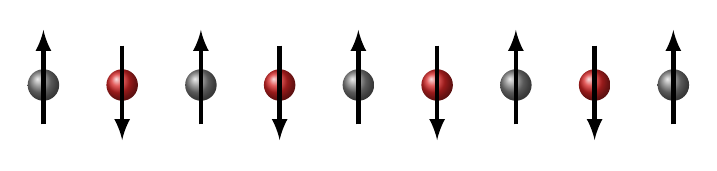
\begin{tikzpicture}
        \tikzstyle{balloon}=[ball color=gray];
        \tikzstyle{balloon2}=[ball color=red!70!gray];
        \foreach\x in {0,2,...,8}{
          \shade[balloon] (\x,0) circle (.2);% node[below right]{$m$};
          \draw[ultra thick,->](\x,-.5)--(\x,.7);
        }
        \foreach\x in {1,3,5,7}{
          \shade[balloon2] (\x,0) circle (.2);% node[below right]{$m$};
          \draw[ultra thick,->](\x,.5)--(\x,-.7);
        }
        
      \end{tikzpicture}\\
      %Ferrimagnetic
    \end{center}
    When they do not cancel, then they can become magnets. This is called
    \textbf{ferromagnetism}:
    \begin{center}
      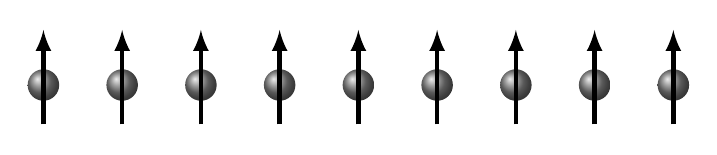
\begin{tikzpicture}
        \tikzstyle{balloon}=[ball color=gray];
        \foreach\x in {0,1,...,8}{
          \shade[balloon] (\x,0) circle (.2);% node[below right]{$m$};
          \draw[ultra thick,->](\x,-.5)--(\x,.7);
        }
      \end{tikzpicture}\\
      %Ferromagnetic
    \end{center}
    Transitional elements such as iron, nickel and cobalt, and their alloys
    will exhibit ferromagnetism.
  \end{enumerate}
\end{frame}



\begin{frame}{Permanent Magnets}
  \begin{enumerate}
    \setcounter{enumi}{3}
  \item The atoms in these ferromagnetic materials are arranged in ``domains''
    wher their magnetic moment is aligned. In the presence of a strong
    external magnetic field, these domains will line up, creating a magnet.
    \begin{center}
      \pic{.6}{domain}
    \end{center}
  \end{enumerate}
\end{frame}


    
\begin{frame}{Earth}
  Earth is also a ``permanent'' magnet, with the \emph{magnetic south pole}
  located near the geographic north pole, and the \emph{magnetic north pole}
  located near the geographic south pole. The poles are tilted by
  $\approx\ang{11}$ from the spin axis.
  \begin{center}
    \pic{.5}{mearthbar}
  \end{center}
  The exact nature of Earth's magnetic field is not known, although it may be
  related to ``generator effect'' from Earth's rotation, circulating the
  outer-core fluid around.
\end{frame}


\section{Magnetic Force}

\begin{frame}{So What Does the Magnetic Field Do?}{In Classical Physics}
  \begin{columns}
    \column[t]{.3\textwidth}
    \begin{center}
      Gravitational Field $\bm{g}$
    \end{center}
    \begin{itemize}
    \item Generated by massive objects
    \item Affects massive objects
    \end{itemize}

    \column[t]{.3\textwidth}
    \begin{center}
      Electric Field $\bm{E}$
    \end{center}
    \begin{itemize}
    \item Generated by charged particles
    \item Affects charged particles
    \end{itemize}

    \column[t]{.4\textwidth}
    \begin{center}
      Magnetic Field $\bm{B}$
    \end{center}
    \begin{itemize}
    \item Generated by \emph{moving} charged particles
    \item Affects moving charged particles
    \end{itemize}
  \end{columns}
\end{frame}



\begin{frame}{Lorentz Force Law}
  Since a moving charge or current create both electric and magnetic fields,
  another moving charge is therefore affected by both $\bm{E}$ and $\bm{B}$.
  The total effect is given by the \textbf{Lorentz force law}:

  \eq{-.2in}{
    \boxed{\bm{F}=q(\bm{E}+\bm{v}\times\bm{B})}
  }

  \vspace{-.1in}$\bm{F}_q=q\bm{E}$ is the electrostatic force, and
  $\bm{F}_M=q\bm{v}\times\bm{B}$ is the magnetic force.
  \begin{center}
    \begin{tabular}{l|c|c}
      \rowcolor{pink}
      \textbf{Quantity} & \textbf{Symbol} & \textbf{SI Unit} \\ \hline
      Total force on the moving charge & $\bm{F}$ & \si{\newton} \\
      Charge                 & $q$      & \si{\coulomb} \\
      Velocity of the charge & $\bm{v}$ & \si{\metre\per\second} \\
      Magnetic field         & $\bm{B}$ & \si{\tesla} \\
      Electric field         & $\bm{E}$ & \si{\newton\per\coulomb}
    \end{tabular}
  \end{center}
\end{frame}



\begin{frame}{Force on a Current-Carrying Conductor in a Magnetic Field}
  Likewise, $\bm{B}$ exerts a force on another current-carrying conductor.

  \eq{-.2in}{
    \boxed{F_M=\bm{I}\ell\times\bm{B}}
  }
  \begin{center}
    \begin{tabular}{l|c|c}
      \rowcolor{pink}
      \textbf{Quantity} & \textbf{Symbol} & \textbf{SI Unit} \\ \hline
      Magnetic force on the conductor   & $\bm{F}_M$ & \si{\newton} \\
      Electric current in the conductor & $\bm{I}$   & \si{\ampere} \\
      Length of the conductor           & $\ell$     & \si{\metre} \\
      Magnetic field                    & $\bm{B}$   & \si{\tesla}
    \end{tabular}
  \end{center}
\end{frame}



\begin{frame}{Magnetic Force on Two Current-Carrying Wires}
  \begin{columns}
    \column{.26\textwidth}
    \pic{1.08}{wirefor}

    \column{.74\textwidth}
    Two parallel current-carrying wires of length $L$ are at a distance $r$
    apart. Magnetic field at wire $2$ from current $I_1$ has constant strength
    along the wire, given by:

    \eq{-.2in}{
      B=\frac{\mu_0I_1}{2\pi r}
    }

    The force of $B$ on $I_2$ is:

    \eq{-.3in}{
      F=I_2LB=\frac{\mu_0I_1I_2L}{2\pi r}
      \;\rightarrow\;
      \boxed{\frac{F}{L}=\frac{\mu_0I_1I_2}{2\pi r}}
    }

    \vspace{-.1in}$I_1$ also exerts the same force on $I_2$, pulling the wires
    toward each other. (We should expect this because of the third law of
    motion.)
  \end{columns}
\end{frame}



\begin{frame}{Circular Motion Caused by a Magnetic Field}
  When a charged particle enters a magnetic field at right angle\ldots
  \begin{itemize}
  \item Magnetic force $\bm{F}_M$ perpendicular to both velocity $\bm{v}$ and
    magnetic field $\bm{B}$.
  \item Results in circular motion
  \end{itemize}
  Centripetal force $\bm{F}_c$ is provided by the magnetic force $\bm{F}_M$.
  Equating the two expressions:

  \eq{-.2in}{
    \frac{mv^2}{r}=qvB
  }
  
  We can solve for $r$ get the radius for a charge with a known
  mass, or solve for mass $m$ of a charged particle based on its radius:  

  \eq{-.2in}{
    r = \frac{mv}{qB}\quad\quad\quad m=\frac{qrB}{v}
  }
\end{frame}



\begin{frame}{DC Motor}
  \begin{center}
    \pic{.35}{simple-motor}
  \end{center}
  \begin{itemize}
  \item When a current runs through the magnetic field formed by the magnets
    (called \textbf{field magnets} or \textbf{stators}), a force is applied
    to the wire, causing the motor to turn
  \item The brushes are connected to a DC power source
  \item The commutators switch current direction every
    \ang{180} to keep it turning
  \item The armature will have hundreds or thousands of coils
  \end{itemize}
\end{frame}



\begin{frame}{Galvanometer}
  \begin{columns}
    \column{.3\textwidth}
    \centering
    \pic1{800px-Galvanometer_diagram}

    \column{.7\textwidth}
    Analog \textbf{voltmeters} and \textbf{ammeters} are based on a
    \textbf{galvanometer} which uses the magnetic force acting on a current.
    \begin{itemize}
    \item Current flows through the coil (\textcolor{red}{red})
    \item External magnetic field applies a force on the wire
    \item The coil rotates
    \item The torque exerted on the coil is balanced by the restoring spring
      (\textcolor{green}{green})
    \end{itemize}
  \end{columns}
\end{frame}



\section{Faraday's Law}

\begin{frame}{Magnetic Flux}
  \textbf{Question:} If a current-carrying wire can generate a magnetic field,
  can a magnetic field affect the current in a wire?

  \vspace{.3in}\textbf{Answer:} Yes, sort of\ldots

  \vspace{.3in}To understand how to \emph{induce} a current by a magnetic field,
  we need to look at ``fluxes''.
\end{frame}



\begin{frame}{Magnetic Flux}
  \begin{columns}
    \column{.45\textwidth}
    \pic1{flux2}
  
    \column{.55\textwidth}

    \vspace{.2in}The strict mathematical definition (i.e.\ using calculus) of
    \textbf{magnetic flux} is defined as:
    
    \eq{-.15in}{
      \boxed{\Phi_M=\int\bm{B}\cdot d\bm{A}}
    }
    
    where $\bm{B}$ is the magnetic field, and $d\bm{A}$ is the infinitesimal
    area pointing \emph{outward}. For a uniform magnetic field, this is
    simplied to (no calculus!):

    \eq{-.2in}{
      \Phi_M=\bm{B}\cdot\bm{A}
    }
  \end{columns}
\end{frame}



\begin{frame}{Magnetic Flux Over a Closed Surface}
  The unit for magnetic flux is a ``weber'' (\si{\weber}), in honor of German
  physicist Wilhelm Weber, who invented the electromagnetic telegraph with Carl
  Gauss:

  \eq{-.3in}{
    \SI1{\weber}=\SI1{\tesla\metre\squared}
  }
  
  The magnetic flux over a closed surface is always zero,
  indicating that magnetic field lines can neither have beginnings nor ends.

  \eq{-.2in}{
    \oint\bm{B}\cdot d\bm{A}=0
  }
\end{frame}


\begin{frame}{Changing Magnetic Flux}
  Changes to magnetic flux can be due to a number of reasons:
  \begin{enumerate}
  \item\textbf{Changing magnetic field}\ldots if the magnetic field is created
    by a time-dependent source (e.g.\ alternating current)
  \item\textbf{Changing orientation of magnetic field} because the
    surface area is moving relative to the magnetic field.
  \item\textbf{Changing area} the surface area from which the flux is
    calculated is changing.
  \end{enumerate}
\end{frame}



\begin{frame}{When Magnetic Flux is Changing}
  \begin{itemize}
  \item When the magnetic flux $\Phi_M$ is changing, an electromotive force
    (\emph{emf}, $\mathcal{E}$) is created in the wire.
  \item Unlike in a circuit, where the \emph{emf} is concentrated at the
    terminals of the battery, the induced \emph{emf} is spread across the
    entire wire.
    \item Since \emph{emf} is work per unit charge, that means that there is an
      electric field inside the wire to move the charges.
    \end{itemize}
\end{frame}


\begin{frame}{Faraday's Law}
  Faraday's law states that the rate of change of magnetic flux produces an
  electromotive force:

  \eq{-.2in}{
    \boxed{
      \overline{\mathcal{E}}={\color{red}{-}}\frac{\Delta\Phi_M}{\Delta t}
    }
  }
  
  The negative sign {\textcolor{red}{highlighted in red}} is the result of
  Lenz's law, which is related to the conservation energy
\end{frame}



\begin{frame}{AC Generators}
  A simple AC (alternating current) generator makes use of the fact that a 
  coil rotating against a fixed magnetic field has a changing flux.
  \begin{center}
    \pic{.45}{generator}
  \end{center}
  Let's say the permanent magnets produce a uniform magnetic field $B$, and the
  coil between them has $N$ turns, and an area $A$. Now let's say that the coil
  is rotating with an angular frequency $\omega$.
\end{frame}



\begin{frame}{AC Generators}
  \begin{columns}
    \column{.35\textwidth}
    \pic{1}{generator}

    \column{.65\textwidth}
    When the coil is turning at a constant rate $\omega$, the angle between the
    coil and the magnetic field is:
    
    \eq{-.2in}{
      \theta=\omega t+\theta_0
    } 

    \vspace{-.1in}where $\theta_0$ is the initial angle (not very important
    coneptually). The magnetic flux through the coil is:
    
    \vspace{-.4in}{\Large
      \begin{align*}
        \Phi_M&=NBA\cos\theta\\
        &=NBA\cos(\omega t+\theta_0)
      \end{align*}
    }
    
    \vspace{-.3in}as the coil turns.
  \end{columns}
\end{frame}



\begin{frame}{AC Generators}
  \begin{columns}
    \column{.33\textwidth}
    \pic{1.05}{generator}

    \column{.67\textwidth}  
    The electromotive force \emph{emf} produced is therefore the rate of change
    of the magnetic flux:

    \eq{-.2in}{
      \mathcal{E}
      =\underbracket{NBA\omega}_{\mathcal{E}_0}\sin(\omega t+\delta)
    }
  \end{columns}
\end{frame}



\begin{frame}{Motional EMF}
  {What happens when I slide the rod to the right?}
  \begin{columns}
    \column{.45\textwidth}
    \pic{1}{motional-emf-1}

    \column{.55\textwidth}
    When sliding the rod to the right with speed $v$, the magnetic flux through
    the loop (and its rate of change) is:

    \vspace{-.4in}{\Large
      \begin{align*}
        \Phi_M     &=BA=B\ell x\\
        \mathcal{E}&=B\ell v
      \end{align*}
    }
    
    \vspace{-.3in}We can use the Lorentz force law on the charges on the rod to
    find the direction of the current $I$.
  \end{columns}
\end{frame}



\begin{frame}{Motional EMF}{What happens when I slide the rod to the right?}
  \begin{columns}
    \column{.22\textwidth}
    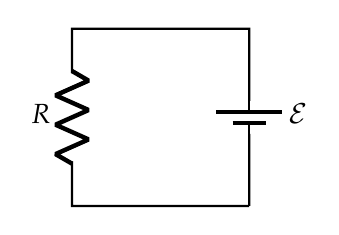
\begin{tikzpicture}[scale=1.5]
      \draw[thick](1.5,0) to[battery1,l_=$\mathcal{E}$] (1.5,1.5)--(0,1.5)
      to[R,l_=$R$] (0,0)--(1.5,0);
    \end{tikzpicture}
    
    \column{.78\textwidth}
    \begin{itemize}
    \item An equivalent circuit is shown on the left
    \item The amount of current can be found using Ohm's law: $V=IR$
    \item Note that the ``motional emf'' produced is spread over the entire
      circuit
      \begin{itemize}
      \item In constrast, in a voltaic cell (or battery), the \emph{emf} is
        concentrated between the two terminals.
      \end{itemize}
    \end{itemize}
  \end{columns}
\end{frame}



\section{Lenz's Law}

\begin{frame}{Lenz's Law}
  Something very interesting happens when the current starts running on the
  wire.
  \begin{center}
    \pic{.35}{motional-emf-2}
  \end{center}
  It produces an ``induced magnetic field'' out of the page, in the opposite
  direction as the field that generated the current in the first place.
\end{frame}



\begin{frame}{Lenz's Law}
  \begin{center}
    \fbox{
      \begin{minipage}{.7\textwidth}
        \textbf{LENZ'S LAW}\\
        The induced \emph{emf} and induced current are in such are
        direction as to oppose the change that produces them
      \end{minipage}
    }
  \end{center}

  \vspace{.2in}So basically, the conservation of energy
\end{frame}
\end{document}
